\documentclass{standalone}
\usepackage{tikz}
\usetikzlibrary{patterns, positioning}
\usepackage[sfdefault]{ClearSans} %% option 'sfdefault' activates Clear Sans as the default text font
\usepackage[T1]{fontenc}

\begin{document}
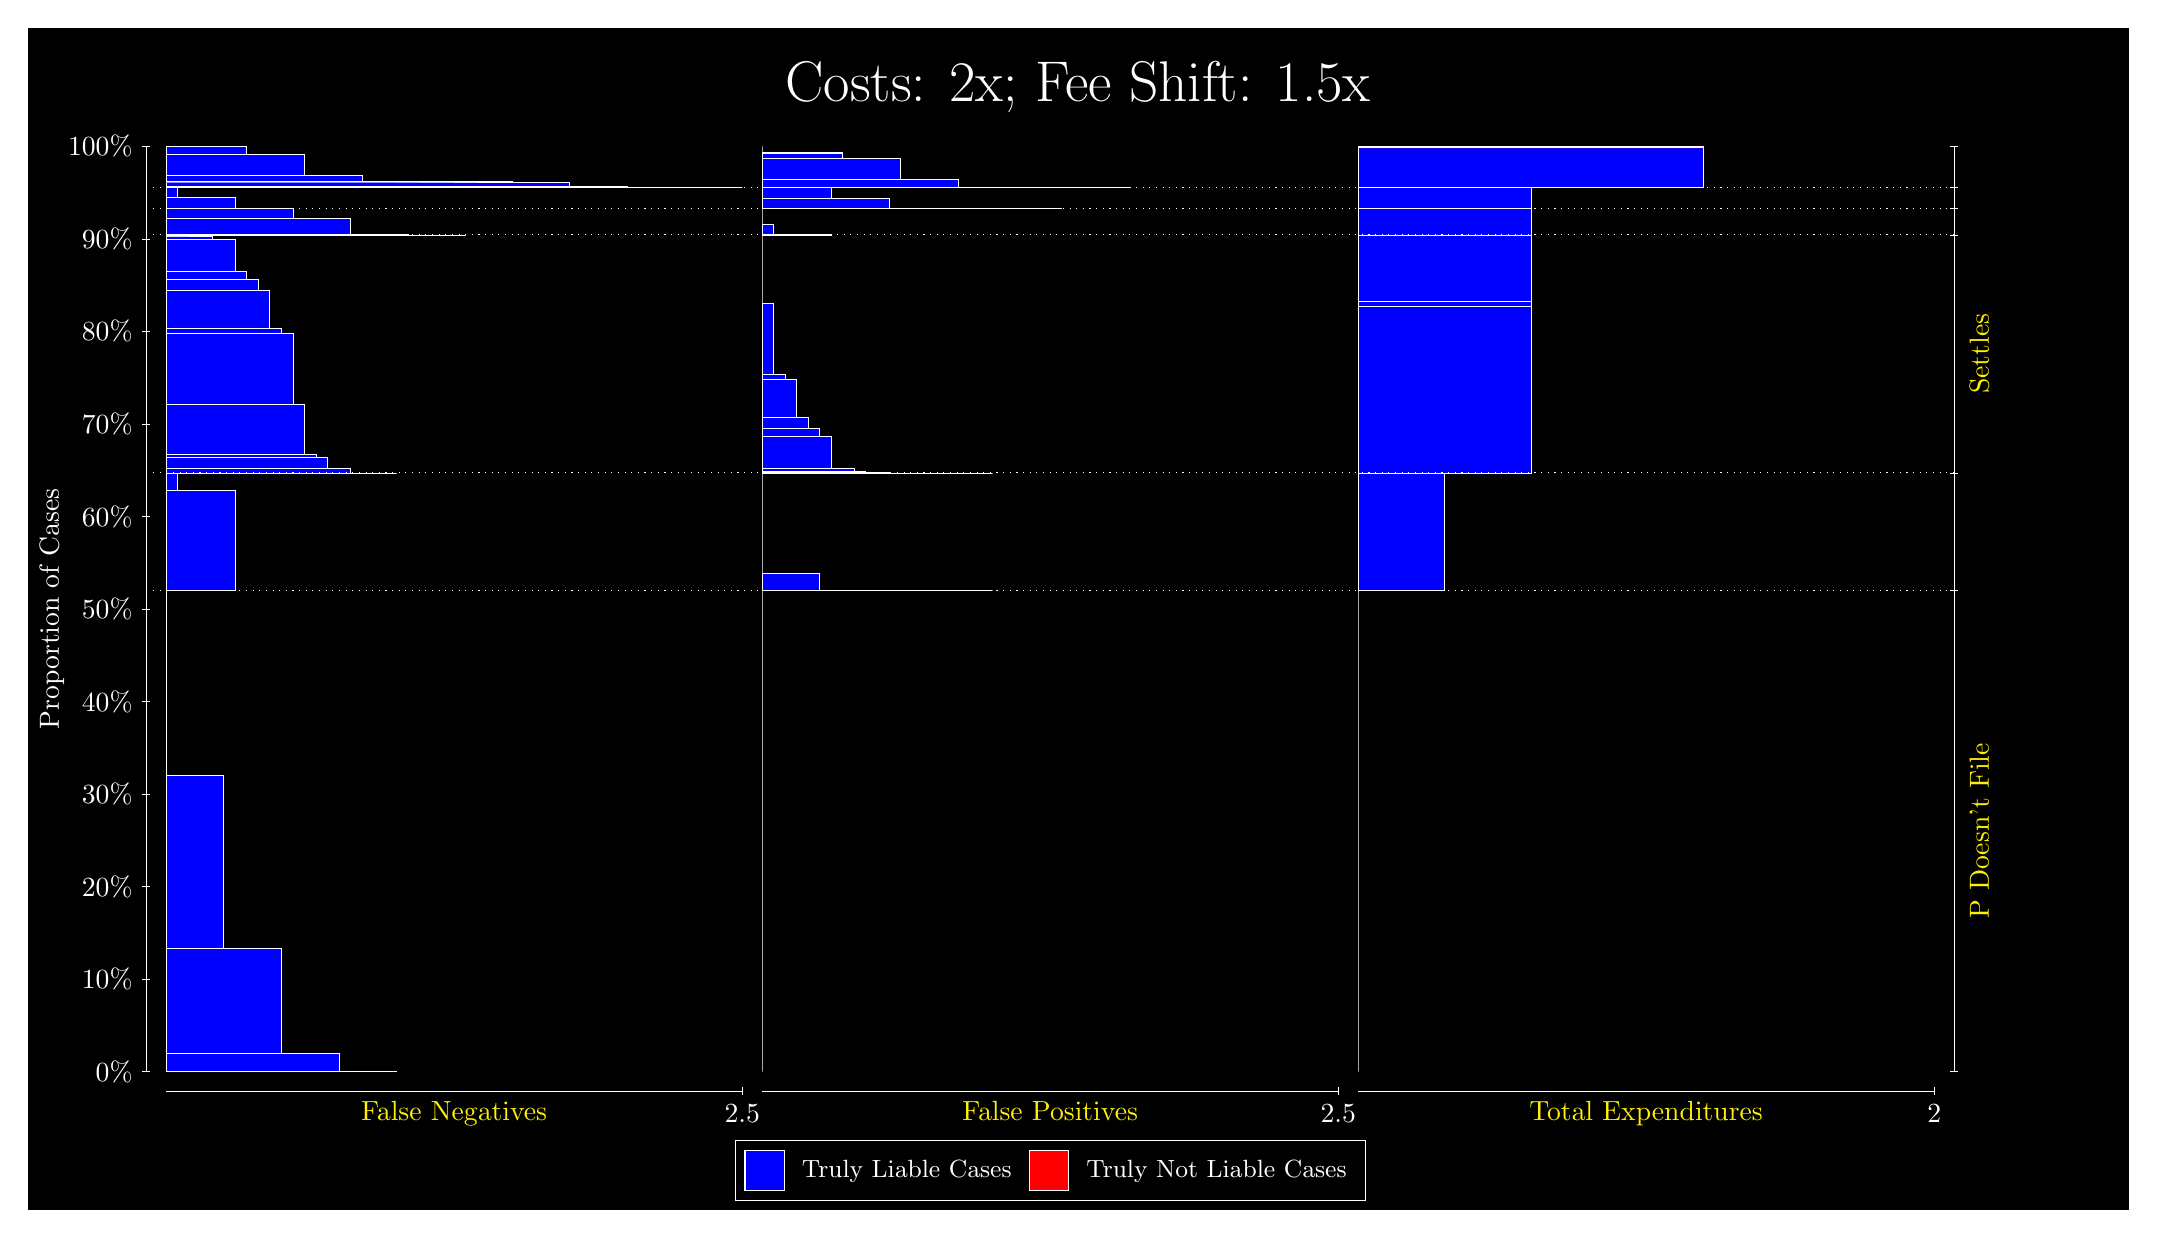
\begin{tikzpicture}
\draw[fill=black] (0,0) rectangle (26.667,15);
\draw[text=white] (0,13.5) rectangle (26.667,15) node[midway] {\huge Costs: 2x; Fee Shift: 1.5x};
\draw[white, very thin] (1.5,1.75) -- (1.5,13.5);
\node[rotate=90, text=white, anchor=center] at (0.3, 7.625) {Proportion of Cases};
\draw[white, very thin] (1.45,1.75) -- (1.55,1.75);
\node[text=white, anchor=east] at (1.45, 1.75) {0\%};
\draw[white, very thin] (1.45,2.925) -- (1.55,2.925);
\node[text=white, anchor=east] at (1.45, 2.925) {10\%};
\draw[white, very thin] (1.45,4.1) -- (1.55,4.1);
\node[text=white, anchor=east] at (1.45, 4.1) {20\%};
\draw[white, very thin] (1.45,5.275) -- (1.55,5.275);
\node[text=white, anchor=east] at (1.45, 5.275) {30\%};
\draw[white, very thin] (1.45,6.45) -- (1.55,6.45);
\node[text=white, anchor=east] at (1.45, 6.45) {40\%};
\draw[white, very thin] (1.45,7.625) -- (1.55,7.625);
\node[text=white, anchor=east] at (1.45, 7.625) {50\%};
\draw[white, very thin] (1.45,8.8) -- (1.55,8.8);
\node[text=white, anchor=east] at (1.45, 8.8) {60\%};
\draw[white, very thin] (1.45,9.975) -- (1.55,9.975);
\node[text=white, anchor=east] at (1.45, 9.975) {70\%};
\draw[white, very thin] (1.45,11.15) -- (1.55,11.15);
\node[text=white, anchor=east] at (1.45, 11.15) {80\%};
\draw[white, very thin] (1.45,12.325) -- (1.55,12.325);
\node[text=white, anchor=east] at (1.45, 12.325) {90\%};
\draw[white, very thin] (1.45,13.5) -- (1.55,13.5);
\node[text=white, anchor=east] at (1.45, 13.5) {100\%};

\draw[white, very thin] (24.457,1.75) -- (24.457,13.5);
\draw[white, very thin] (24.407,1.75) -- (24.507,1.75);
\node[anchor=west] at (24.407, 1.75) {};
\draw[white, very thin] (24.407,7.8593) -- (24.507,7.8593);
\node[anchor=west] at (24.407, 7.8593) {};
\draw[white, very thin] (24.407,9.3534) -- (24.507,9.3534);
\node[anchor=west] at (24.407, 9.3534) {};
\draw[white, very thin] (24.407,12.376) -- (24.507,12.376);
\node[anchor=west] at (24.407, 12.376) {};
\draw[white, very thin] (24.407,12.715) -- (24.507,12.715);
\node[anchor=west] at (24.407, 12.715) {};
\draw[white, very thin] (24.407,12.981) -- (24.507,12.981);
\node[anchor=west] at (24.407, 12.981) {};
\draw[white, very thin] (24.407,13.5) -- (24.507,13.5);
\node[anchor=west] at (24.407, 13.5) {};

\draw[white, very thin, fill=blue] (1.75,1.75) rectangle (4.6775,1.7523);
\draw[white, very thin, fill=blue] (1.75,1.7523) rectangle (3.9457,1.9774);
\draw[white, very thin, fill=blue] (1.75,1.9774) rectangle (3.2138,3.3122);
\draw[white, very thin, fill=blue] (1.75,3.3122) rectangle (2.4819,5.5108);
\draw[white, very thin, fill=red] (1.75,5.5108) rectangle (1.75,5.5108);
\draw[white, very thin, fill=blue] (1.75,5.5108) rectangle (1.75,7.8593);
\draw[white, very thin, fill=blue] (1.75,7.8593) rectangle (2.6283,9.1293);
\draw[white, very thin, fill=blue] (1.75,9.1293) rectangle (1.8964,9.3525);
\draw[white, very thin, fill=red] (1.75,9.3525) rectangle (1.75,9.3525);
\draw[white, very thin, fill=blue] (1.75,9.3525) rectangle (1.75,9.3534);
\draw[white, very thin, fill=blue] (1.75,9.3534) rectangle (4.6775,9.3534);
\draw[white, very thin, fill=blue] (1.75,9.3534) rectangle (4.3848,9.3535);
\draw[white, very thin, fill=blue] (1.75,9.3535) rectangle (4.092,9.4057);
\draw[white, very thin, fill=blue] (1.75,9.4057) rectangle (3.9457,9.4091);
\draw[white, very thin, fill=blue] (1.75,9.4091) rectangle (3.7993,9.5556);
\draw[white, very thin, fill=blue] (1.75,9.5556) rectangle (3.6529,9.5891);
\draw[white, very thin, fill=blue] (1.75,9.5891) rectangle (3.5065,10.224);
\draw[white, very thin, fill=blue] (1.75,10.224) rectangle (3.3602,11.131);
\draw[white, very thin, fill=blue] (1.75,11.131) rectangle (3.2138,11.194);
\draw[white, very thin, fill=blue] (1.75,11.194) rectangle (3.0674,11.669);
\draw[white, very thin, fill=blue] (1.75,11.669) rectangle (2.921,11.809);
\draw[white, very thin, fill=blue] (1.75,11.809) rectangle (2.7746,11.913);
\draw[white, very thin, fill=blue] (1.75,11.913) rectangle (2.6283,12.318);
\draw[white, very thin, fill=blue] (1.75,12.318) rectangle (2.4819,12.321);
\draw[white, very thin, fill=blue] (1.75,12.321) rectangle (2.3355,12.361);
\draw[white, very thin, fill=blue] (1.75,12.361) rectangle (2.1891,12.367);
\draw[white, very thin, fill=blue] (1.75,12.367) rectangle (2.0428,12.367);
\draw[white, very thin, fill=blue] (1.75,12.367) rectangle (1.8964,12.376);
\draw[white, very thin, fill=red] (1.75,12.376) rectangle (1.75,12.376);
\draw[white, very thin, fill=blue] (1.75,12.376) rectangle (1.75,12.376);
\draw[white, very thin, fill=blue] (1.75,12.376) rectangle (5.5558,12.376);
\draw[white, very thin, fill=blue] (1.75,12.376) rectangle (4.8239,12.382);
\draw[white, very thin, fill=blue] (1.75,12.382) rectangle (4.092,12.584);
\draw[white, very thin, fill=blue] (1.75,12.584) rectangle (3.3602,12.714);
\draw[white, very thin, fill=blue] (1.75,12.714) rectangle (2.6283,12.715);
\draw[white, very thin, fill=red] (1.75,12.715) rectangle (1.75,12.715);
\draw[white, very thin, fill=blue] (1.75,12.715) rectangle (2.6283,12.856);
\draw[white, very thin, fill=blue] (1.75,12.856) rectangle (1.8964,12.979);
\draw[white, very thin, fill=red] (1.75,12.979) rectangle (1.75,12.979);
\draw[white, very thin, fill=blue] (1.75,12.979) rectangle (1.75,12.981);
\draw[white, very thin, fill=blue] (1.75,12.981) rectangle (9.0689,12.981);
\draw[white, very thin, fill=blue] (1.75,12.981) rectangle (8.337,12.981);
\draw[white, very thin, fill=blue] (1.75,12.981) rectangle (7.6051,12.993);
\draw[white, very thin, fill=blue] (1.75,12.993) rectangle (6.8732,13.048);
\draw[white, very thin, fill=blue] (1.75,13.048) rectangle (6.1413,13.052);
\draw[white, very thin, fill=blue] (1.75,13.052) rectangle (5.7022,13.052);
\draw[white, very thin, fill=blue] (1.75,13.052) rectangle (5.4094,13.052);
\draw[white, very thin, fill=blue] (1.75,13.052) rectangle (4.9703,13.052);
\draw[white, very thin, fill=blue] (1.75,13.052) rectangle (4.6775,13.052);
\draw[white, very thin, fill=blue] (1.75,13.052) rectangle (4.2384,13.127);
\draw[white, very thin, fill=blue] (1.75,13.127) rectangle (3.5065,13.399);
\draw[white, very thin, fill=blue] (1.75,13.399) rectangle (2.7746,13.496);
\draw[white, very thin, fill=blue] (1.75,13.496) rectangle (2.0428,13.5);
\draw[white, very thin, fill=red] (1.75,13.5) rectangle (1.75,13.5);
\draw[white, very thin, fill=blue] (1.75,13.5) rectangle (1.75,13.5);
\draw[white, very thin, fill=red] (9.3189,1.75) rectangle (9.3189,1.75);
\draw[white, very thin, fill=blue] (9.3189,1.75) rectangle (9.3189,7.8593);
\draw[white, very thin, fill=red] (9.3189,7.8593) rectangle (12.246,7.8593);
\draw[white, very thin, fill=blue] (9.3189,7.8593) rectangle (12.246,7.8593);
\draw[white, very thin, fill=blue] (9.3189,7.8593) rectangle (11.515,7.8593);
\draw[white, very thin, fill=blue] (9.3189,7.8593) rectangle (10.783,7.8602);
\draw[white, very thin, fill=blue] (9.3189,7.8602) rectangle (10.051,8.0834);
\draw[white, very thin, fill=blue] (9.3189,8.0834) rectangle (9.3189,9.3534);
\draw[white, very thin, fill=red] (9.3189,9.3534) rectangle (12.246,9.3534);
\draw[white, very thin, fill=blue] (9.3189,9.3534) rectangle (12.246,9.3534);
\draw[white, very thin, fill=red] (9.3189,9.3534) rectangle (11.954,9.3534);
\draw[white, very thin, fill=blue] (9.3189,9.3534) rectangle (11.954,9.3534);
\draw[white, very thin, fill=red] (9.3189,9.3534) rectangle (11.661,9.3534);
\draw[white, very thin, fill=blue] (9.3189,9.3534) rectangle (11.661,9.3534);
\draw[white, very thin, fill=blue] (9.3189,9.3534) rectangle (11.515,9.3534);
\draw[white, very thin, fill=red] (9.3189,9.3534) rectangle (11.368,9.3534);
\draw[white, very thin, fill=blue] (9.3189,9.3534) rectangle (11.368,9.3534);
\draw[white, very thin, fill=blue] (9.3189,9.3534) rectangle (11.222,9.3534);
\draw[white, very thin, fill=red] (9.3189,9.3534) rectangle (11.075,9.3534);
\draw[white, very thin, fill=blue] (9.3189,9.3534) rectangle (11.075,9.3534);
\draw[white, very thin, fill=blue] (9.3189,9.3534) rectangle (10.929,9.3625);
\draw[white, very thin, fill=blue] (9.3189,9.3625) rectangle (10.783,9.3627);
\draw[white, very thin, fill=blue] (9.3189,9.3627) rectangle (10.636,9.3687);
\draw[white, very thin, fill=blue] (9.3189,9.3687) rectangle (10.49,9.4083);
\draw[white, very thin, fill=blue] (9.3189,9.4083) rectangle (10.344,9.4117);
\draw[white, very thin, fill=blue] (9.3189,9.4117) rectangle (10.197,9.8172);
\draw[white, very thin, fill=blue] (9.3189,9.8172) rectangle (10.051,9.921);
\draw[white, very thin, fill=blue] (9.3189,9.921) rectangle (9.9044,10.061);
\draw[white, very thin, fill=blue] (9.3189,10.061) rectangle (9.758,10.536);
\draw[white, very thin, fill=blue] (9.3189,10.536) rectangle (9.6116,10.599);
\draw[white, very thin, fill=blue] (9.3189,10.599) rectangle (9.4652,11.506);
\draw[white, very thin, fill=blue] (9.3189,11.506) rectangle (9.3189,12.376);
\draw[white, very thin, fill=red] (9.3189,12.376) rectangle (10.197,12.376);
\draw[white, very thin, fill=blue] (9.3189,12.376) rectangle (10.197,12.378);
\draw[white, very thin, fill=blue] (9.3189,12.378) rectangle (9.4652,12.508);
\draw[white, very thin, fill=blue] (9.3189,12.508) rectangle (9.3189,12.715);
\draw[white, very thin, fill=red] (9.3189,12.715) rectangle (13.125,12.715);
\draw[white, very thin, fill=blue] (9.3189,12.715) rectangle (13.125,12.715);
\draw[white, very thin, fill=blue] (9.3189,12.715) rectangle (12.393,12.715);
\draw[white, very thin, fill=blue] (9.3189,12.715) rectangle (11.661,12.717);
\draw[white, very thin, fill=blue] (9.3189,12.717) rectangle (10.929,12.84);
\draw[white, very thin, fill=blue] (9.3189,12.84) rectangle (10.197,12.981);
\draw[white, very thin, fill=red] (9.3189,12.981) rectangle (14.003,12.981);
\draw[white, very thin, fill=blue] (9.3189,12.981) rectangle (14.003,12.981);
\draw[white, very thin, fill=red] (9.3189,12.981) rectangle (13.271,12.981);
\draw[white, very thin, fill=blue] (9.3189,12.981) rectangle (13.271,12.981);
\draw[white, very thin, fill=red] (9.3189,12.981) rectangle (12.539,12.981);
\draw[white, very thin, fill=blue] (9.3189,12.981) rectangle (12.539,12.985);
\draw[white, very thin, fill=blue] (9.3189,12.985) rectangle (11.807,13.081);
\draw[white, very thin, fill=red] (9.3189,13.081) rectangle (11.807,13.081);
\draw[white, very thin, fill=blue] (9.3189,13.081) rectangle (11.807,13.081);
\draw[white, very thin, fill=blue] (9.3189,13.081) rectangle (11.075,13.353);
\draw[white, very thin, fill=blue] (9.3189,13.353) rectangle (11.075,13.354);
\draw[white, very thin, fill=blue] (9.3189,13.354) rectangle (10.344,13.414);
\draw[white, very thin, fill=blue] (9.3189,13.414) rectangle (10.344,13.429);
\draw[white, very thin, fill=red] (9.3189,13.429) rectangle (9.9044,13.429);
\draw[white, very thin, fill=blue] (9.3189,13.429) rectangle (9.9044,13.429);
\draw[white, very thin, fill=blue] (9.3189,13.429) rectangle (9.6116,13.429);
\draw[white, very thin, fill=blue] (9.3189,13.429) rectangle (9.6116,13.429);
\draw[white, very thin, fill=red] (9.3189,13.429) rectangle (9.3189,13.429);
\draw[white, very thin, fill=blue] (9.3189,13.429) rectangle (9.3189,13.5);
\draw[white, very thin, fill=red] (16.888,1.75) rectangle (16.888,1.75);
\draw[white, very thin, fill=blue] (16.888,1.75) rectangle (16.888,7.8593);
\draw[white, very thin, fill=red] (16.888,7.8593) rectangle (17.986,7.8593);
\draw[white, very thin, fill=blue] (16.888,7.8593) rectangle (17.986,9.3534);
\draw[white, very thin, fill=red] (16.888,9.3534) rectangle (19.083,9.3534);
\draw[white, very thin, fill=blue] (16.888,9.3534) rectangle (19.083,11.466);
\draw[white, very thin, fill=red] (16.888,11.466) rectangle (19.083,11.466);
\draw[white, very thin, fill=blue] (16.888,11.466) rectangle (19.083,11.536);
\draw[white, very thin, fill=red] (16.888,11.536) rectangle (19.083,11.536);
\draw[white, very thin, fill=blue] (16.888,11.536) rectangle (19.083,12.376);
\draw[white, very thin, fill=red] (16.888,12.376) rectangle (19.083,12.376);
\draw[white, very thin, fill=blue] (16.888,12.376) rectangle (19.083,12.715);
\draw[white, very thin, fill=red] (16.888,12.715) rectangle (19.083,12.715);
\draw[white, very thin, fill=blue] (16.888,12.715) rectangle (19.083,12.981);
\draw[white, very thin, fill=red] (16.888,12.981) rectangle (21.279,12.981);
\draw[white, very thin, fill=blue] (16.888,12.981) rectangle (21.279,13.484);
\draw[white, very thin, fill=red] (16.888,13.484) rectangle (21.279,13.484);
\draw[white, very thin, fill=blue] (16.888,13.484) rectangle (21.279,13.5);
\draw[white, dotted] (1.5,7.8593) -- (24.457,7.8593);
\draw[white, dotted] (1.5,9.3534) -- (24.457,9.3534);
\draw[white, dotted] (1.5,12.376) -- (24.457,12.376);
\draw[white, dotted] (1.5,12.715) -- (24.457,12.715);
\draw[white, dotted] (1.5,12.981) -- (24.457,12.981);
\draw[white, very thin] (1.75,1.5) -- (9.0689,1.5);
\node[text=yellow, anchor=north] at (5.4094, 1.5) {False Negatives};
\draw[white, very thin] (9.0689,1.45) -- (9.0689,1.55);
\node[text=white, anchor=north] at (9.0689, 1.45) {2.5};

\draw[white, very thin] (9.3189,1.5) -- (16.638,1.5);
\node[text=yellow, anchor=north] at (12.978, 1.5) {False Positives};
\draw[white, very thin] (16.638,1.45) -- (16.638,1.55);
\node[text=white, anchor=north] at (16.638, 1.45) {2.5};

\draw[white, very thin] (16.888,1.5) -- (24.207,1.5);
\node[text=yellow, anchor=north] at (20.547, 1.5) {Total Expenditures};
\draw[white, very thin] (24.207,1.45) -- (24.207,1.55);
\node[text=white, anchor=north] at (24.207, 1.45) {2};

\node[text=yellow, centered, rotate=90] at (24.777, 4.8047) {P Doesn't File};

\node[text=yellow, centered, rotate=90] at (24.777, 10.865) {Settles};




\draw (12.978300999999998,1.5) node[draw=none] (baseCoordinate) {};
\begin{scope}[align=center]
        \matrix[scale=0.5, draw=white, below=0.5cm of baseCoordinate, nodes={draw}, column sep=0.1cm]{
            \node[rectangle, draw, minimum width=0.5cm, minimum height=0.5cm, fill=blue] {}; &
            \node[draw=none, font=\small, text=white] (B) {Truly Liable Cases}; &
            \node[rectangle, draw, minimum width=0.5cm, minimum height=0.5cm, fill=red] {}; &
            \node[draw=none, font=\small, text=white] (B) {Truly Not Liable Cases}; \\
            };
\end{scope}

\end{tikzpicture}
\end{document}